\documentclass[12pt]{article}

\usepackage{graphicx}
\graphicspath{ {./images/} }
\usepackage{amsmath}

\usepackage{listings}

\usepackage{ragged2e}
\justifying
\usepackage[onehalfspacing]{setspace}
\usepackage[margin=2.5cm]{geometry}

\usepackage[ngerman]{babel}

\title{Ausarbeitung - KW Signal}
\author{Julian Thiele, 70476743}

\begin{document}
\sloppy

\maketitle
\newpage
\tableofcontents
\newpage

\section{Einleitung}
Wir betrachten einen Benzinverbrennungsmotor mit einem Drehzahlbereich von 800 U/min bis 6000 U/min.
Um die Drehzahl zu messen ist über einem Geberad der Kurbelwelle ein Induktiv- oder Hallsensor angebracht.
Das Geberad besitzt 36 Zähne mit einer Zahnlücke von 2 Zähnen.
Durch die 36 Zähne erhält man eine Auflösung von 10° pro Zahn.
Der erste Zahn nach der Zahnlücke liegt bei 0°. Dadurch fehlen die Zähne bei 340° und 350°.

Die Daten des Sensors werden an die GPIO Ports des AT91SAM7 Prozessors weitergeleitet, welcher die Daten bearbeitet.
Durch den Prozessor soll die Drehzahl und Position des Motors bestimmt werden und mit den Daten
ein Impuls für die Zündung der Zündkerze im Motor generiert werden.

\section{Berechnungen}
Hier sind die wesentlichen Berechnungen, auf deren Grundage die Timer konfiguriert werden.\newline\newline
Bezeichner:\newline
Drehzahl $D$, mit $D_{min} = 800 U/min$ und $D_{max} = 6000 U/min$ \newline
Master-Clock Frequenz $f_{MSTCLK} = 48MHz$ \newline
Zeit $t$ \newline


\subsection{Minimale und Maximale Zeit zwischen zwei Zähnen}

Berechnung der Zeit pro Zahn:
\begin{gather}
    D = \frac{1}{t} \Leftrightarrow t_{Umdrehung} = \frac{1}{D} \Leftrightarrow t_{Zahn} = \frac{1}{D * 36}
\end{gather}
Minimale Zeit pro Zahn:
\begin{gather}
    t_{Zahn,min} = \frac{1}{D_{max} * 36} = \frac{1}{6.000 * 36}min = 
    \frac{60.000}{6.000 * 36}ms \approx 0,28ms
\end{gather}
Maximale Zeit pro Zahn:
\begin{gather}
    t_{Zahn,max} = \frac{1}{D_{min} * 36} = \frac{1}{800 * 36}min = 
    \frac{60.000}{800 * 36}ms \approx 2,08ms
\end{gather}

\subsection{Berechnung der Frequenzen}

Maximal Benötigte Zeit in der Zahnlücke:
\begin{gather}
    t_{Luecke,max} = t_{Zahn,max} * 3 = 6,24ms
\end{gather}
Maximale Frequenz für die Lücke bei 16-bit:
\begin{gather}
    f_{Luecke, max} = \frac{2^{16}}{t_{Luecke,max}} = \frac{2^{16}}{6,24ms} \approx 10,5 MHz
\end{gather}
Maximale Frequenz für eine Umdrehung bei 16-bit:
\begin{gather}
    f_{Umdrehung,max} = \frac{2^{16}}{t_{Zahn,max} * 36} = \frac{2^{16}}{75ms} \approx 0,9MHz
\end{gather}
Mögliche Clock Frequenzen:
\begin{itemize}
    \item $f_{CLK1} = f_{MSTCLK} / 2 = 48MHz / 2 = 24MHz$ \\
    \item $f_{CLK2} = f_{MSTCLK} / 8 = 48MHz / 8 = 6MHz$ \\
    \item $f_{CLK3} = f_{MSTCLK} / 32 = 48MHz / 32 = 1,5MHz$ \\
    \item $f_{CLK4} = f_{MSTCLK} / 128 = 48MHz / 128 = 375kHz$ \\
    \item $f_{CLK5} = f_{MSTCLK} / 1024 = 48MHz / 1024 = 46,875kHz$ \\
\end{itemize}

\subsection{Berechnung der Impulslänge}
Maximaler Wert im Counter Register zwischen einem Zahn:
\begin{gather}
    n_{CMP} = t_{Zahn,max} * f_{CLK2} = 2,08ms * 6MHz = 12.480
\end{gather}
Maximale Impulslänge:
\begin{gather}
    n_{I} = 2^{16} - 12.480 = 53.056
\end{gather}


\section{Bestimmung der Zahnlücke}
\subsection{Vorgang}
Das Zahnrad besitzt 36 Zähne, mit einer Zahnlücke von 2 Zähnen.
Um die Zahnlücke zu bestimmen, muss das Intervall zwischen zwei Zähnen betrachtet werden.
Passiert die Zahnlücke den Sensor, erhält man ein Zeitintervall, das ungefähr 3 mal so lang ist, wie das
Intervall zwischen den restlichen Zähen.
Die Zähne können mithilfe von steigenden Flanken im Eingangssignal identifiziert werden.
Das Zeitintervall wird mit einem Timer gemessen, dem ein Compare Wert zugewiesen wird.
Dieser Timer wird bei jeder steigenden Flanke zurückgesetzt, wodurch die Zeitintervalle gemessen werden.
Den Compare Wert kann man entsprechend des Letzten Intervalls wählen. Wird der Compare Wert von dem Timer erreicht,
hat man die Zahnlücke erreicht.

Man muss jedoch beachten, dass sich die Zeitintervalle während einer Umdrehung mehrfach verändern,
aufgrund von Zündungen in anderen Kolben.
Deshalb sollte der Compare-Wert nicht zu dicht an dem zuvor gemessenen Intervall liegen. 
Im Gegenzug dazu sollte der Wert auch nicht zu hoch gewählt werden. Sonst könnte durch kürzere Intervalle während der
Zahnlücke, diese nicht detektiert werden.

Man sollte eine Intervall von ungefähr dem Doppelten der vorherigen Perioden wählen, um zu beiden Seiten hin einen
Puffer zu haben.

\subsection{Konfiguration}
Um den Timer für die Zeiterfassung zu Konfigurieren muss als erstes der entsprechende GPIO Pin als Eingang konfiguriert werden.
Für den Timer wird Channel 3 gewählt dementsprechend muss die Clock für den Channel 3 im Power Management Controller (PMC) aktivert werden.

Als erstes wird des Channel Mode Register konfiguriert.
Dieser Timer soll im Capture Mode betrieben werden. Das \textit{WAVE-Bit (Bit 15)} muss dementsprechend auf 0 gesetzt werden.
Als Clock wird \textit{TIMER\_CLOCK2} genutzt, da diese die höchste Auflösung bietet, ohne dass es bei der
maximalen länge der Lücke zu einem Overflow kommt. Dafür muss in das \textit{TCCLKS-Feld (Bit 0-2)} des Registers der Wert $001_{2}$ geschrieben werden.
Da der Timer dauerhaft laufen soll, muss der Burst-Mode deaktiviert werden, indem das \textit{BURST-Feld (Bit 4-5)} auf $00_{2}$ gesetzt wird.

Der Counter Wert des Timers soll bei jedem Zahn zurückgesetzt werden und vorher in das Capture Register A gelesen werden. 
Dafür muss zunächst das \textit{LDRA-Feld (Bit 16-17)} mit $01_{2}$ beschrieben werden, um bei jeder steigenden Flanke den Counter-Wert in das Register zu schreiben.
Um den Counter zurückzusetzten, muss die Rising-Edge des TIOA als externer Trigger genutzt werden.
Dafür muss das \textit{ETRGEDG-Feld (Bit 8-9)} auf $01_2$ und das \textit{ABETRG-Bit (Bit 10)} auf $1$ gesetzt werden.

Damit das Capture Register A jedes mal beschrieben wird, muss dieses nach jedem Zahn gelesen werden.
Dafür muss der External Trigger Interrupt aktiviert werden, indem im Interrupt Enable Register \textit{TC\_IER} der \textit{ETRGS-Bit (Bit 7)} auf 1 gesetzt wird.

Um nun den Zeitpunkt der Zahnlücke zu bekommen, muss noch der RC Compare Interrupt aktiviert werden.
Dafür wird im im Interrupt Enable Register \textit{TC\_IER} zusätzlich das \textit{CPCS-Bit (Bit 4)} auf 1 gesetzt.

\subsection{Interrupt Service Routine}
Als erstes muss in der ISR geprüft werden, durch was der Interrupt ausgelöst wurde.
Dazu werden die Bits im im TC Status Register \textit{TC\_SR} überprüft.
Steht das \textit{ETRGS-Bit (Bit 7)} auf 1, muss das Capture Register A gelesen und den Compare Wert in Register C auf das jeweilig 2-fache des Wertes gesetzt werden.
Steht das \textit{CPCS-Bit (Bit 4)} auf 1, ist die Zahnlücke gerade an oberster Stelle.

\section{Bestimmung der Drehzahl}
\subsection{Funktion}
Es gibt mehrere Möglichkeiten, die Drehzahl zu bestimmen.

\subsubsection{Möglichkeit 1}
Um die Drehzahl zu bestimmen, kann die Zeit zwischen den Zähnen gemessen werden. Diese Zeit sind 10° der gesamten Umdrehung.
Multipliziert man diese Zeit mit 36 erhält man dementsprechend die Zeit für eine Umdrehung.
Aus dieser Zeit kann im Anschluss die Drehzahl berechnet werden.

Zudem ist die Implementierung dieser Methode sehr simpel, da man das Intervall zwischen zwei Zähnen bereits gemessen wird.
Man muss lediglich in der ISR für die Bestimmung der Zahnlücke beim Auftreten des externen Trigger Interrupts den Wert des
Capture Registers A lesen und daraus die Zeit zwischen den beiden Zähnen berechnen. 

Das Problem dieser Methode ist, dass durch die Zündung in anderen Kolben die Zeit zwischen zwei Zähnen
innerhalb einer Umdrehung schwanken kann. Durch diese Ungenauigkeit kann die Drehzahl stark schwanken.

\subsubsection{Möglichkeit 2}
Eine weitere Möglichkeit ist, die Zeit der gesamten Umdrehung zu messen.
Während der gesamten Umdrehung gleichen sich die Schwankungen, die bei Möglichkeit 1 ein Problem dargestellt haben,
gegenseitig aus.
Für die Umsetzung wird ein weiterer Timer benötigt, der die Zeit zwischen zwei Zahnlücken misst.
Die gemessene Zeit für eine Umdrehung kann im Anschluss in die Drehzahl umgerechnet werden.

Aufgrund der höheren Konsitenz wird diese Möglichkeit hier umgesetzt.

\subsection{Konfiguration}
Anfangs muss die Clock im PMC für den Timer Channel 0 aktiviert werden, welcher für diesen Counter genutzt wird.
Der Channel wird mit dem Capture Mode verwendet. Dafür wird das \textit{WAVE-Bit (Bit 15)} im Counter Mode Register auf 0 gesetzt.
Das \textit{TCCLKS-Feld (Bit 0-2)} wird auf $100_2$ gesetzt, um die \textit{TIMER\_CLOCK4} zu verwenden.
Mit dieser Frequenz wird sichergestellt, dass es zu keine Overflow kommt, solange sich der Motor in seinem typischen Drehzahlbereich bewegt.
Außerdem wird das \textit{BURST-Feld (Bit 4-5)} auf $00_2$ gesetzt.


\section{Interrupt Service Routine}
Die Service Routine von Timer3 wird so angepasst, dass bei jeder erkannten Zahnlücke der Wert des Counter Registers von Timer0 ausgelesen
und in einer Variable gespeichert wird. So kann der Wert, außerhalb der ISR, zu weiteren Berechnungen genutzt werden.
Der Counter wird im Anschluss durch das schreiben des \textit{SWTRG-Bit} zurückgesetzt.

\section{Bestimmung der Position}

\subsection{Funktion}
Um die Position zu bestimmen, werden zwei Timer benötigt. Ein Timer wird als Taktsignal genutzt.
Der Timer gibt bei jeder steigenden Flanke des Sensors ein Signal ab, welches von einem anderen Timer
als Clock Signal genutzt wird. So können die Zähne gezählt werden, welche jeweils 10° entsprechen.
Da bei dem ersten Zahnrad nach der Lücke 0° erreicht sind, muss der Timer zurückgesetzt werden, sobal die 
Lücke erreicht wurde.

\subsection{Konfiguration}

Als Signalgeber wird Timer Channel 1 genutzt.
Dieser wird im Channel Mode Register als Wave Mode konfiguriert.
Das \textit{WAVE-Bit (Bit 15)} muss dementsprechend auf 1 gesetzt werden.
Als Clock wird \textit{TIMER\_CLOCK2} genutzt. In das \textit{TCCLKS-Feld (Bit 0-2)} des Registers wird der Wert $001_{2}$ geschrieben werden.
Das \textit{BURST-Feld (Bit 4-5)} wird auf $00_{2}$ gesetzt, da kein Burst Mode genutzt wird.

Da die Steigende Flanke des Eingangs TIOB genutzt werden soll, muss als erstes das externe Event aktiviert werden.
Dazu wird das \textit{EEVT-Feld (Bit 10-11)} im Channel Mode Register auf 0 gesetzt.
Um nun einen Trigger bei steigenden Flanken auszulösen wird in das \textit{EEVTEDG-Bit (Bit 8-9)} mit dem Wert $01_2$ beschrieben.
Das Signal wird auf den Ausgang TIOB2 weitergeleitet, indem das \textit{AEEVT-Feld} auf $01_2$ gesetzt wird.
Um das Signal kurz danach wieder zu deaktivieren, wird das \textit{ENETRG-Bit} auf 1 gesetzt.
Das Compare Register A wird auf einen kleinen Wert gesetzt (z.B. 100). Das \textit{ACAP-Bit} wird auf $10_2$ gesetzt. So wird
das Signal kurz nach der steigenden Flanke von TIOB wieder auf LOW gezogen.

Dieses Signal wird in dem Channel 2 als Clock-Eingang benutzt.
Hierfür muss als erstes das \textit{TC2XC2S} im \textit{TC Block Mode Register} auf $11_2$ gesetzt werden.
Im Anschluss muss in das \textit{TCCLKS-Feld (Bit 0-2)} des \textit{TC Mode Rgister} der Wert $111_2$ geschrieben werden.
Das \textit{WAVE-Bit (Bit 15)} wird auf 0 gesetzt. Das \textit{WAVE-Bit} wird of 0 gesetzt, um den Channel im Compare Mode zu betreiben.

\subsection{Interrupt Service Routine}
Für das Bestimmen der Position wird keine ISR benötigt. Für das Zurücksetzen des Counters muss jedoch die ISR 
beim Erkennen der Zahnlücke angepasst werden. Beim Auftreten des Interrupts muss zusätzlich das Bit \textit{SWTRG}
im \textit{TC Channel Control Register} von Channel 2 auf $1$ gesetzt werden, um den Counter zurück zu setzten.


\section{Generation eines Impulses}

\subsection{Funktion}
Um einen Impuls zu generieren kann ein Timer im WAVE-Mode genutzt werden. 
Der Timer ist inaktiv, bis Timer2 bei der gewünschten Position angelangt ist und das Zahnrad weniger als
10° von der gewünschten Position entfernt ist.
Sobald die Position erreicht ist, wird die Impuls-Generation im one-shot Modus gestartet.
Der Compare-Wert A wird auf den gewünschten Startwert gesetzt, während Compare-Wert C auf den Startwert mit der Periodenlänge addiert gesetzt wird.
Wird der Compare-Wert A erreicht, wird das Ausgangssignal auf \textit{HIGH} gesetzt.
Sobald der Counter bei dem CompareWert C angelangt ist, wird das Signal wieder auf \textit{LOW} gezogen und der Timer 
gestoppt, bis er wieder aktiviert wird. Dadurch werden keine weiteren Signale gesendet.


\subsection{Konfiguration}
Für die Generation eines Impulses wird ein weiterer Channel (Channel 4) benötigt, der durch das schreiben einer $0$ in das 
\textit{WAVE-Bit (Bit 15)} des \textit{TC Channel Mode Register} in WAVE Mode betrieben wird.
Das \textit{TCCLKS-Feld (Feld 0-2)} wird auf $001_2$ gesetzt, um die \textit{TIMER\_CLOCK2} zu nutzen. 
Burst-Mode wird durch den Wert $00_2$ ausgestellt.
Um den Counter beim Erreichen des Compare Registers C zu stoppen, wird das \textit{CPCSTOP-Bit (Bit 6)} auf 1 gesetzt.
Um das Signal zu erzeugen muss das \textit{ACPA-Feld (Bit 16-17)} auf $01_2$ und das \textit{ACPC-Feld (Bit 18-19)} auf $10_2$ gesetzt werden.
Das \textit{WAVSEL-Feld (Bit 13-14)} im \textit{TC Channel Mode Register} wird auf $00_2$ gesetzt. Dadurch wird von unten nach oben gezählt
und von Compare C kein Reset ausgelöst, der den Timer unter ungünstigen Umständen wieder ungewollt starten könnte.

Um den Counter bei gewünschter Position zu aktivieren, muss Timer2 angepasst werden.
In dem \textit{TC Interrupt Enable Register} muss das \textit{CPCS-Bit (bit 4)} auf 1 gesetzt werden.
Damit wird eine ISQ gesendet, sobald die Position erreicht ist. Die Position wird im Compare Register C eingetragen.
Hierbei muss beachtet werden, dass 0° einem Compare Wert von 1 entsprechen, 10° einem Wert von 2 und so weiter. 

\subsection{Interrupt Service Routine}
Als erstes muss die Service Routine von Channel 3 weiter angepasst werden.
Bei jedem Trigger, muss der Wert in einer Variable gespeichert werden. 

In der ISR von Timer2 werden die Werte des Compare Registers A und C gesetzt und im Anschluss
das \textit{SWTRG-Bit (Bit 2)} im \textit{TC Channel Control Register} von Channel 4 auf 1 gesetzt.
Durch den Reset wird Channel 4 neu gestartet, bis der Compare Wert von Register C erreicht wurde.



\newpage
\section{Anhang}
\subsection{Interrupt Service Routines in Pseudocode}

\begin{lstlisting}
void Timer3_ISR()
{
    if(ETRGS)
    {
        global_var_zahn = readTimer3RegisterA();
        global_var_umdrehung = readTimer0RegisterCounter();
        writeTimer3RegisterC(global_var_zahn * 2);
    }
    if(CPCS)
    {
        writeTimer2CCR(SWTRG);
    }
}

void Timer2_ISR()
{
    int winkel_einerstelle = 7;
    writeTimer4RegisterA(global_var_zahn * (winkel_einerstelle/10));
    writeTimer4RegisterC(
        global_var_zahn * (winkel_einerstelle/10) + 100);
    writeTimer4CCR(SWTRG);
}
\end{lstlisting}
\newpage


\begin{figure}
    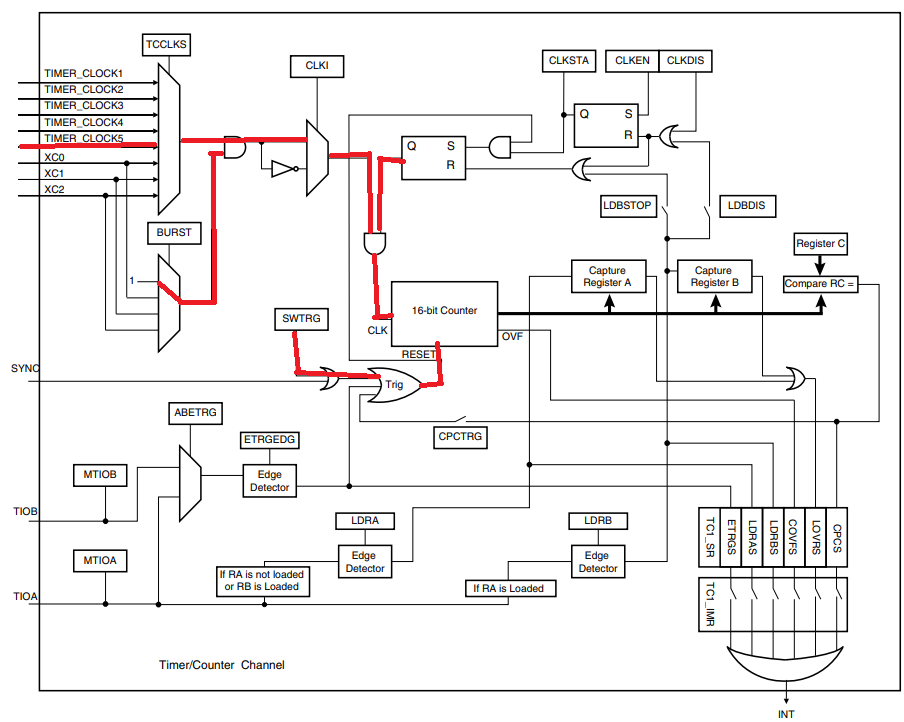
\includegraphics[width=\textwidth]{Timer0.png}
    \caption{Timer0 Konfiguration}
\end{figure}
\begin{figure}
    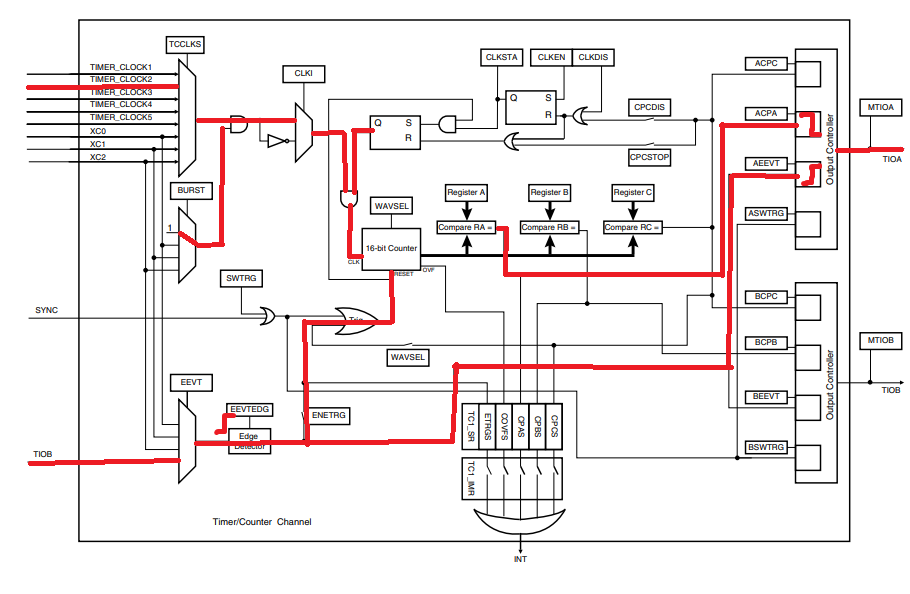
\includegraphics[width=\textwidth]{Timer1.png}
    \caption{Timer1 Konfiguration}
\end{figure}
\begin{figure}
    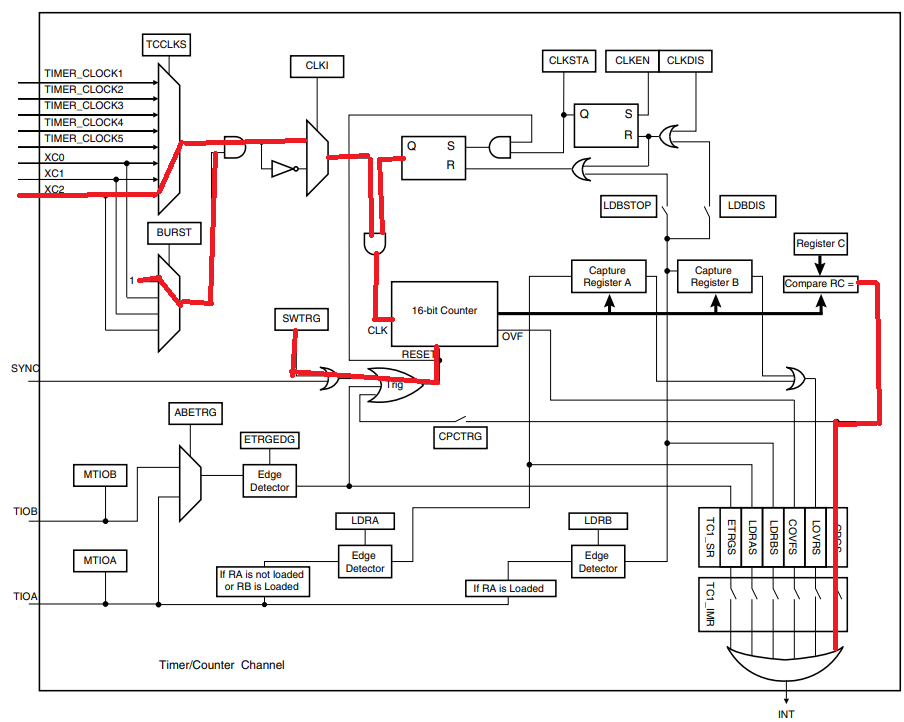
\includegraphics[width=\textwidth]{Timer2.png}
    \caption{Timer2 Konfiguration}
\end{figure}
\begin{figure}
    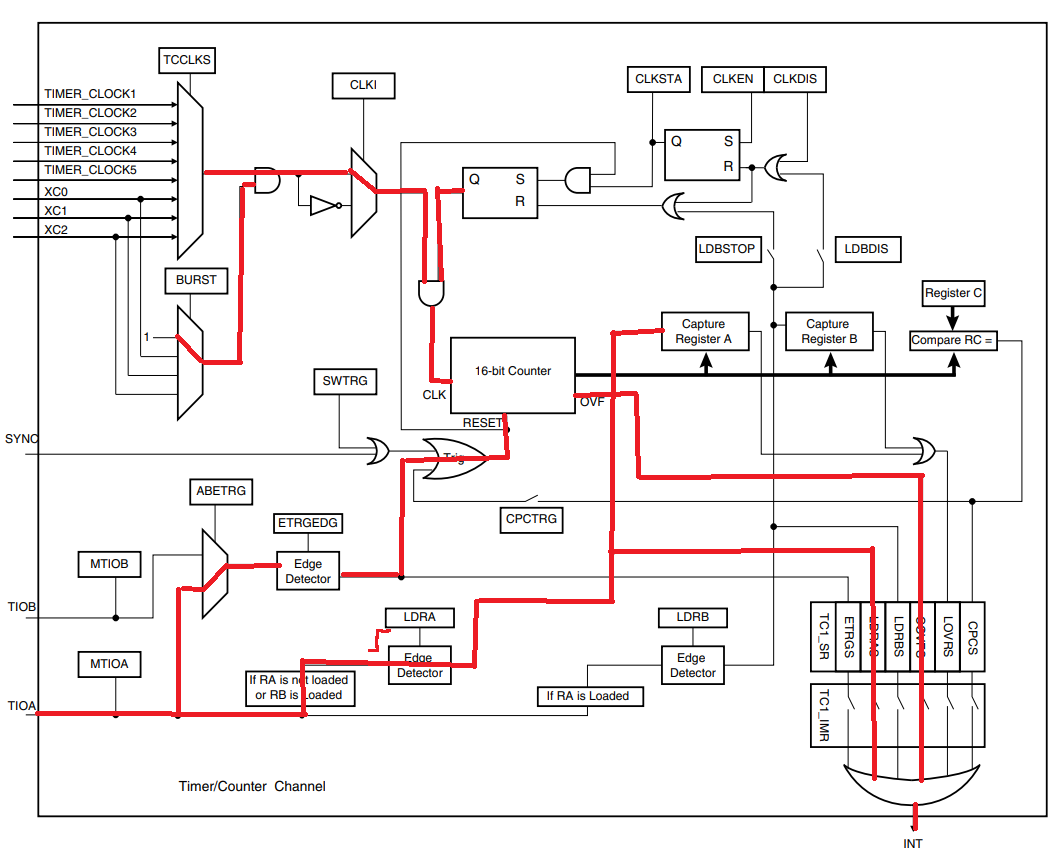
\includegraphics[width=\textwidth]{Timer3.png}
    \caption{Timer3 Konfiguration}
\end{figure}
\begin{figure}
    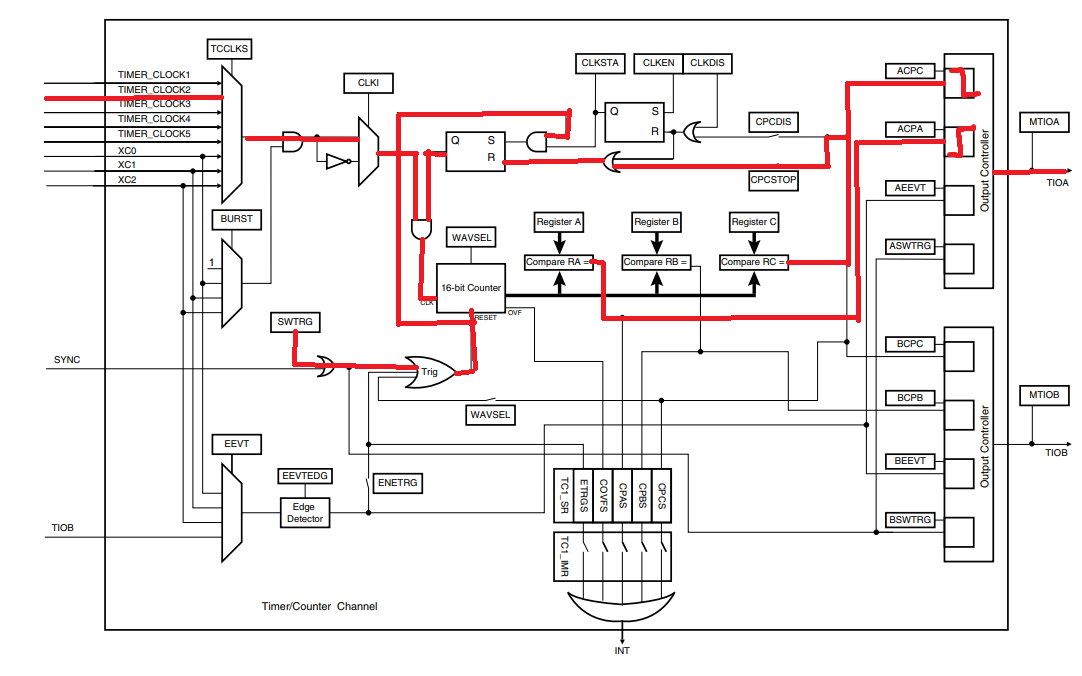
\includegraphics[width=\textwidth]{Timer4.png}
    \caption{Timer4 Konfiguration}
\end{figure}
\begin{figure}
    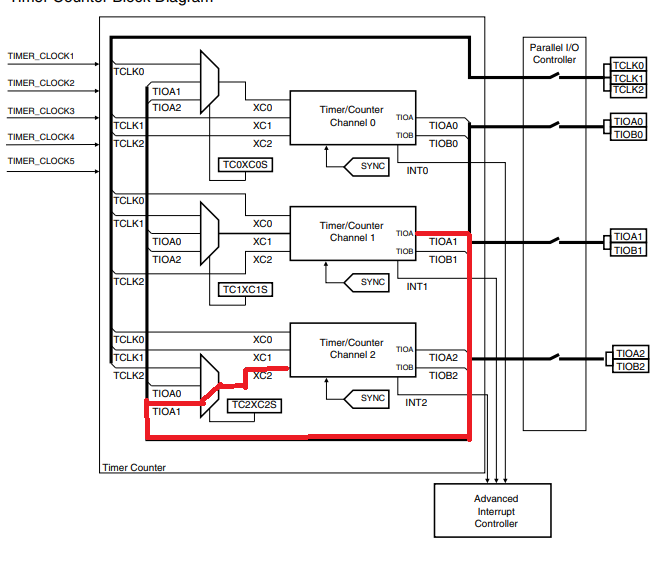
\includegraphics[width=\textwidth]{Timer_Blockschaltbild.png}
    \caption{Timer1 und Timer2 äußere Verdrahtung}
\end{figure}


\end{document}